\section{Identity and Lifecycle Management}\label{sec:security-identity}

The system relies on Keycloak as the central Identity Provider (IdP). 
A dedicated realm was configured to manage practitioners and patients, utilizing specialized clients and custom extensions to ensure a secure registration lifecycle.

\subsection{Keycloak Configuration and Clients}

Keycloak manages three primary OIDC clients: a confidential client used internally by the Backend (BFF) to validate tokens through its middleware, a confidential client for the oauth2 proxy that manages browser sessions, and a public client for mobile devices. 
% Both user-facing (browser and mobile) clients are configured to use the \textbf{Authorization Code Flow with PKCE} to mitigate code interception attacks.
% While PKCE was originally designed to protect the authorization code flow in mobile apps, it's also used with the Browser's confidential client to prevent Authorization Code Injection and to maintain a unified flow throughout the system.
% To align with healthcare standards, Keycloak is configured to map internal user roles to \ac{SMART} on FHIR scopes, which are then embedded as claims within the issued \acp{JWT}.

% It's registration action also maps a static role to the user based on the platform used (practitioner for browser application users, patient for mobile application users)

Both user-facing clients leverage the Authorization Code Flow with PKCE to prevent code interception and authorization injection attacks across all endpoints. 
% To maintain compliance with health informatics standards, Keycloak maps these identity contexts directly to SMART on FHIR scopes embedded natively within the issued token payloads.

\subsection{User Registration and Resource Provisioning}

To maintain synchronization between the identity provider and the healthcare data layer, the system implements an automated provisioning workflow triggered by user registration.

\subsubsection{Keycloak Event Listener}
A custom Keycloak Event Listener is deployed to capture the \texttt{REGISTER} event. Upon execution, the listener performs the following sequence (see Figure~\ref{fig:registration-provisioning-sequence}):
\begin{enumerate}
    \item Obtains a \texttt{client-credentials} access token to authenticate as a trusted service.
    \item Invokes the BFF registration endpoint with the new user's context.
    \item The BFF validates the incoming \ac{JWT} and verifies the caller against a client allowlist stored as secure secrets.
    \item Based on the originating Client ID, the system maps the user to a \ac{FHIR} resource type: \texttt{Practitioner} for web-based signups or \texttt{Patient} for mobile registrations.
\end{enumerate}

\begin{figure}[H]
    \centering
    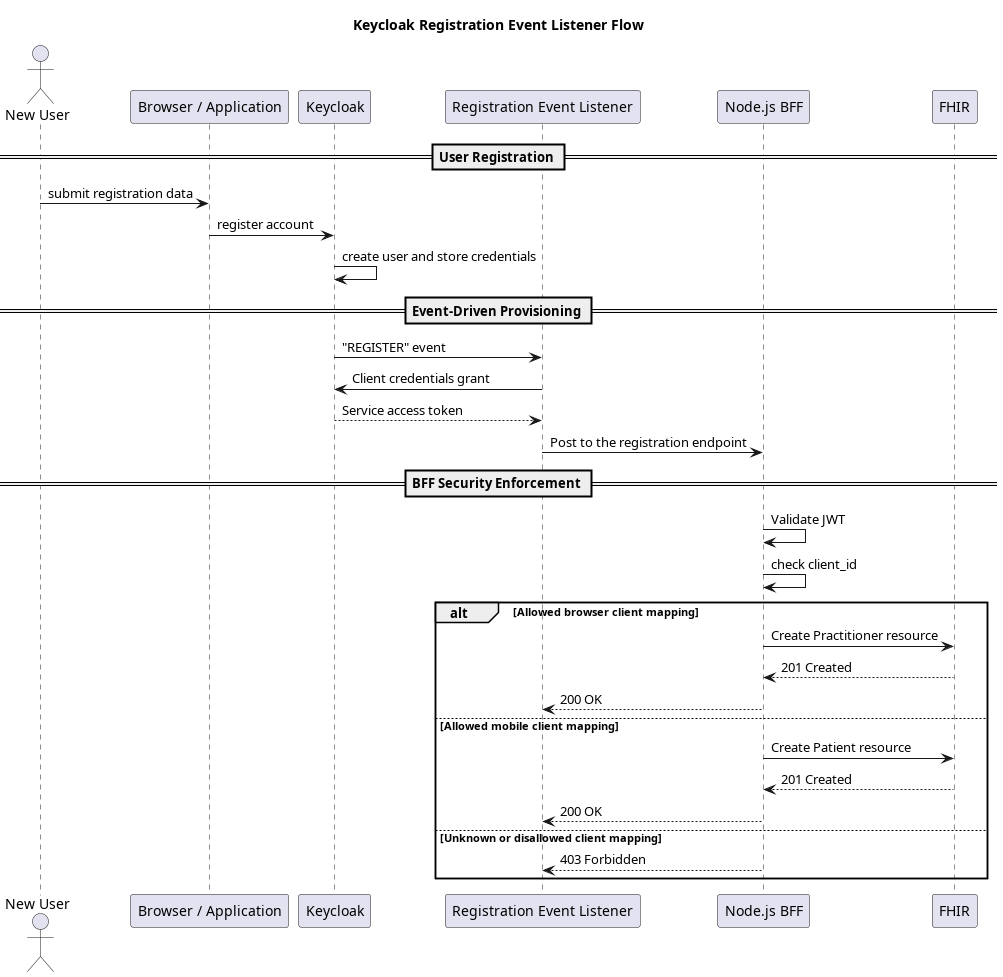
\includegraphics[width=0.92\linewidth]{Security/images/registration-flow-listeners.png}
    \caption{Registration Provisioning Sequence: Event-driven synchronization between Keycloak and the FHIR Resource Server.}
    \label{fig:registration-provisioning-sequence}
\end{figure}

\subsection{Custom Security Extensions (SPIs)}

To strengthen registration integrity, two custom Keycloak Service Provider Interfaces (SPIs) were developed to implement a robust OTP-based email verification mechanism, and support bot mitigation  during the registration lifecycle.

\paragraph{Email OTP Verification (Authenticator SPI)}
This authenticator runs after the registration form has been completed and issues a 6-digit one-time password to the user's email address. 
The code is stored in the authentication session, the user must submit the same value to continue, and a successful match marks the account as email-verified before authentication completes.


\paragraph{Registration CAPTCHA (FormAction SPI)}
The ALTCHA registration extension is a required execution step in the registration flow. 
It generates a challenge from the Keycloak authenticator configuration, renders the challenge to the registration form, and validates the submitted solution before registration can proceed. 
This prevents automated account creation while keeping the CAPTCHA logic inside the Keycloak flow.

\subsection{Persistence Layer}
Identity data, including hashed credentials and role mappings, are persisted in a dedicated PostgreSQL database. This instance is isolated within a private network, accessible only by the Keycloak service.


% \paragraph{Email Code Verification (FormAction SPI)}
% This SPI introduces a mandatory execution step in the registration flow. It validates the user-submitted verification code against a transient value stored in the Keycloak authentication session. If the codes match, the user's email is marked as verified; otherwise, the registration is halted with a validation error.
% It also binds the registration session to a specific out-of-band channel, preventing session hijacking during account creation
% \paragraph{Verification Code Issuance (RealmResourceProvider SPI)}
% This extension provides a secure endpoint for triggering the issuance of one-time codes. It generates a numeric code, stores it as a session note, and dispatches it using Keycloak's internal email templating service. This ensures that the verification logic remains decoupled from the frontend while maintaining strict session binding.


% \subsubsection{Keycloak Realm \& Clients}
% Keycloak is our chosen identity provider, a dedicated realm hosts a client for
% the web application (via the BFF) and a client for mobile usage. For the
% current browser flow, authentication is handled at the gateway using nginx
% \texttt{auth\_request} with \texttt{oauth2-proxy} and Keycloak (Authorization
% Code + PKCE).

% \subsection{Keycloak Configuration}


% \subsubsection{Clients, Scopes}
% The BFF requests valid scopes. Keycloak is be configured to permit these scopes
% for the client based on the user's role and map these roles to appropriate
% SMART scopes.

% \subsubsection{Keycloak-Side Registration Trigger}
% The Keycloak side of registration provisioning is limited to emitting the REGISTER event and invoking the listener extension; full authorization checks and resource mapping are enforced in the backend provisioning endpoint (see Registration Provisioning subsection).

% \subsubsection{Registration Provisioning via Keycloak Event Listener}
% FHIR resource provisioning on user registration is triggered by a custom
% Keycloak Event Listener (\texttt{REGISTER} event). The listener obtains a
% client-credentials access token from Keycloak and calls the backend
% registration endpoint. The following figure shows the provisioning sequence:
% \begin{figure}[H]
%     \centering
%     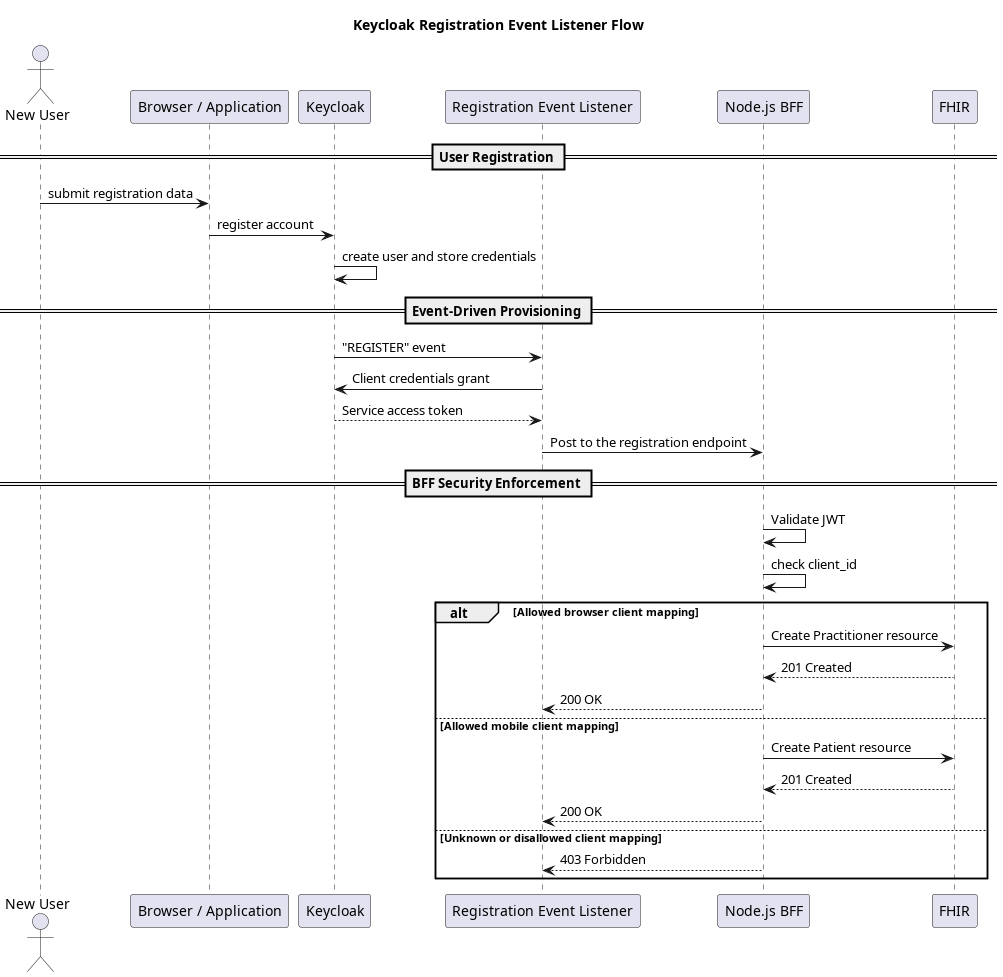
\includegraphics[width=0.92\linewidth]{Security/images/registration-flow-listeners.png}
%     \caption{Registration Provisioning Sequence: Keycloak emits REGISTER event, the Event Listener obtains a client-credentials token, calls the BFF provisioning endpoint, and the BFF enforces JWT and caller allowlist checks before creating the mapped FHIR resource}
%     \label{fig:registration-provisioning-sequence}
% \end{figure}

% The endpoint is protected in two layers:
% \begin{itemize}
%     \item JWT validation (\texttt{requireApiAuth})
%     \item caller client allowlist check (\texttt{requireProvisionerClient})
% \end{itemize}

% Resource type is selected from the registration client ID:
% \begin{itemize}
%     \item \texttt{KC\_BROWSER\_CLIENT\_IDS} $\rightarrow$ \texttt{Practitioner}
%     \item \texttt{KC\_MOBILE\_CLIENT\_IDS} $\rightarrow$ \texttt{Patient}
% \end{itemize}
% Unknown mappings are rejected with HTTP 400

% \subsubsection{Custom Keycloak SPIs for Registration Email Verification}
% To strengthen registration integrity, we added two custom Keycloak SPIs in a dedicated verify-email extension: a FormAction SPI and a RealmResourceProvider SPI. Together, they introduce an email-code verification step during registration and a backend endpoint to issue verification codes.

% \paragraph{SPI 1: FormAction SPI (Registration Email Code Verification)}
% The custom FormAction is registered through a FormActionFactory and appears as a required registration execution. Its purpose is to validate a user-entered email verification code against the expected value stored in the current Keycloak authentication session.
% On successful validation, the registration continues and the user email is marked as verified in the registration flow context. On mismatch, the flow fails with a validation error and prompts the user to re-enter a valid code.

% \paragraph{SPI 2: RealmResourceProvider SPI (Email Code Issuance Endpoint)}
% The custom RealmResourceProvider exposes an extension endpoint used during registration to send a one-time verification code. The provider:
% \begin{itemize}
% \item validates the client context before issuing a code,
% \item resolves the active authentication session,
% \item generates a numeric one-time code,
% \item stores the code as an authentication session note,
% \item sends the code using Keycloak email templating.
% \end{itemize}
% The implementation includes explicit error handling for invalid client identifiers and missing authentication sessions.


% \subsection{Credentials PostgreSQL}
% Keycloak's backing database, storing user accounts, roles, and credentials.
